
In this section, we take a close look at the proposed structure and capabilities of the framework, Imagine.
We will then discuss the implementation and its difficulties.

\section{Proposed Functionality}

The framework shall have two primary capabilities: first, it should enable fast and easy access to the 3D pose calculated from the detected marker.
Second, given a digital 3d model to display, it should be capable of returning a rendering of the object within the scene on top of the live preview, correctly positioned.

Generally, the framework shall work as in the following.
Once the framework is running, OpenCV reads the camera frame directly from the camera.
This frame is copied to the worker threads that will detect markers.
The original unaltered frame is passed back up to be shown as the background of the later rendering.

These worker threads are where the computational expensive part of actually detecting the marker happens.
Using the OpenCV for Android library, we detect markers and calculate their three dimensional pose.
All detected markers are put into a list with the important attached information, such as the corresponding identification number of the detected marker.

This list is passed back to the main controlling element of the framework.
Here it can be passed directly to listening classes if that option was chosen.
This is done when only the marker information is required and not a rendering.
If not, the list is filtered for only those markers that the user wants to track.
These trackables have to have been registered beforehand by the user.
Then the model information is attached to all detected trackable assets and passed down to the rendering part of the framework.
Here, this filtered and supplemented list is used to render all objects onto the correct positions with the correct perspective modifications on top of the camera image.

Apart from the above mentioned basic functionality capabilities, the framework should also handle the easy gathering of performance and error information, mainly by extending the relevant functions of Android.
This can include gathering the logs to a listener, bypassing the Android logging mechanism, and any further functionality that could be useful.

\begin{figure}
	\centering
	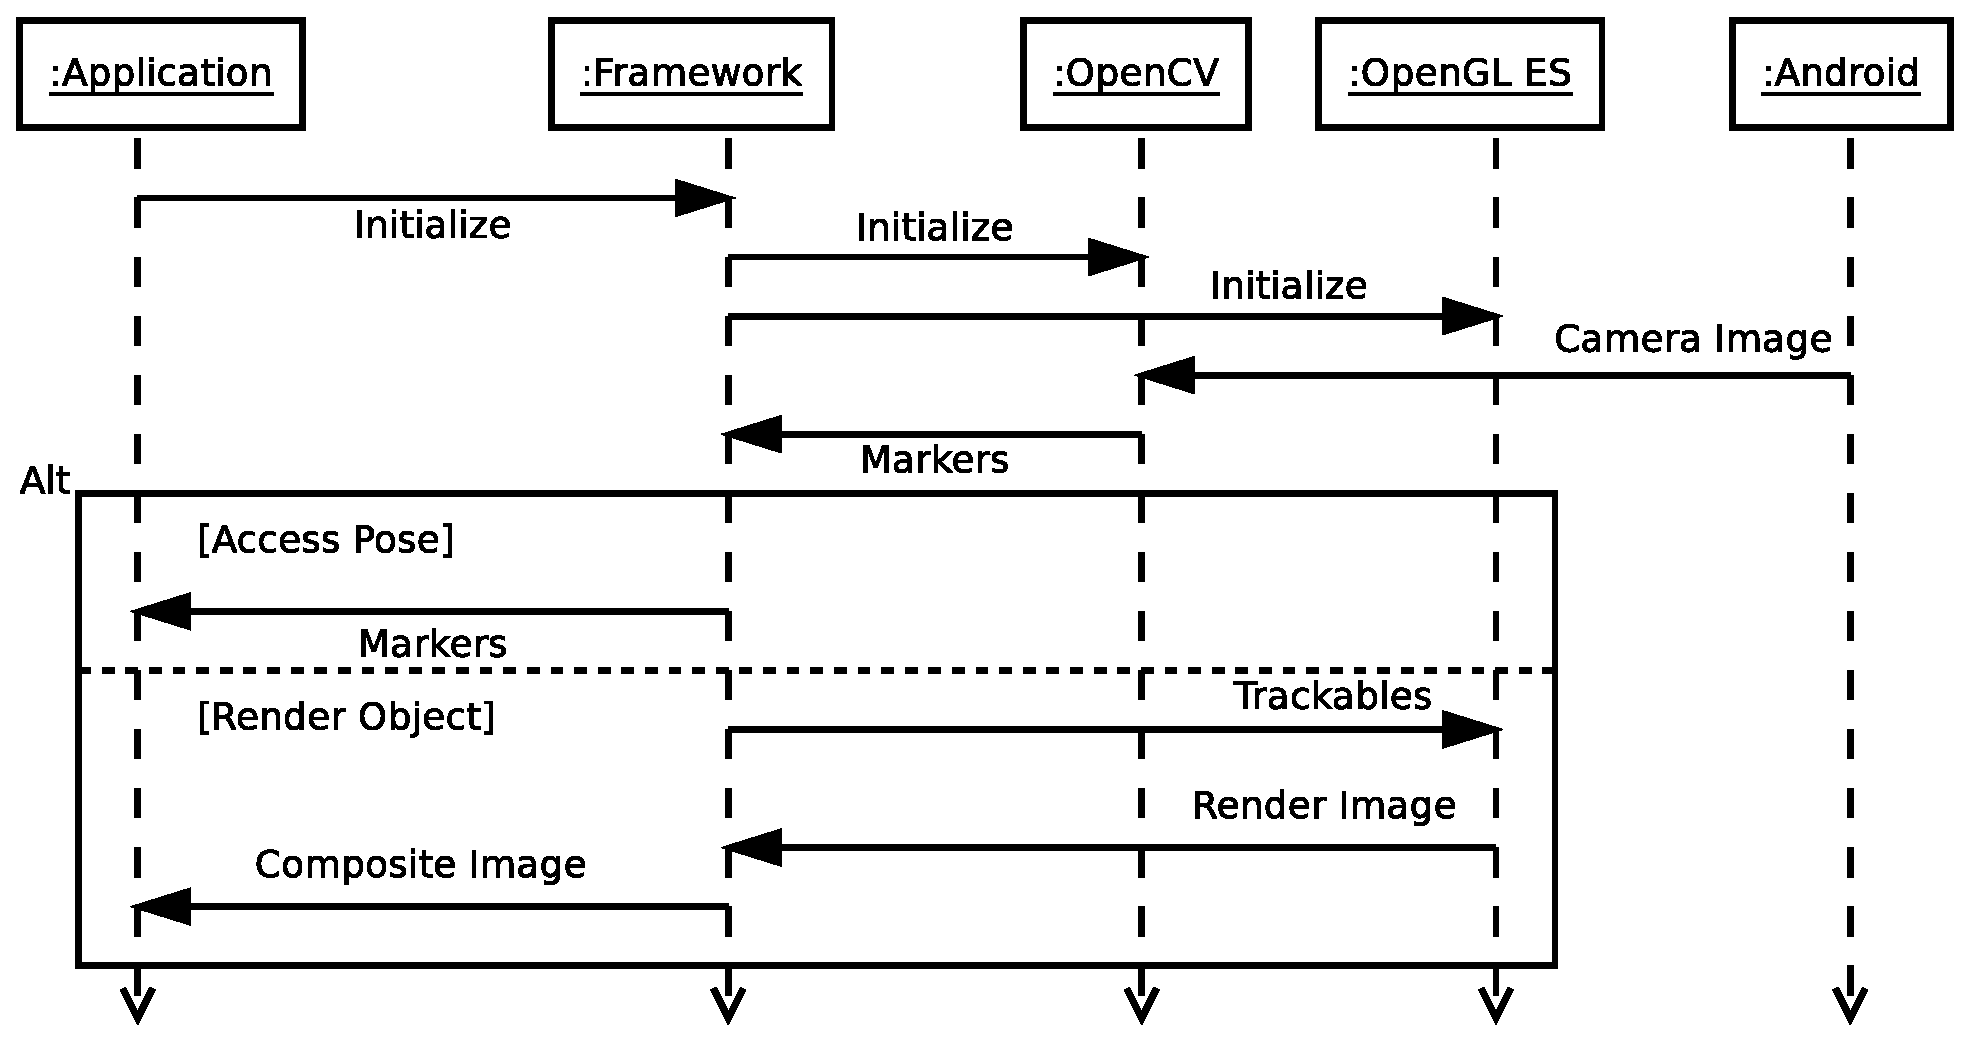
\includegraphics[width=12cm]{img/sequence_access.eps}
	\caption[Access Sequence.]{The proposed sequence of the workflow with the framework, using OpenCV for Android and OpenGL ES.}
	\label{fig:sequence_access}
\end{figure}

Figure \ref{fig:sequence_access} shows the proposed sequence of events of Imagine, and where data can be input or read.
As proposed, the framework should offer a wide variety of uses, without being overly complex from an outside perspective.
Another important aspect we want to make possible is the possibility of changing all the more important parameters during runtime, such as switching the model or adding a new marker.
This should allow a less restrictive usage of the framework and any derived apps as a result.

\section{Dependencies}

Primary dependency is of course an Android environment, given that it is the target platform for the framework.
The framework is written in Java with Android specific syntax and structure.
Aside from the basic requirements, the framework will depend mainly on two external software solutions.

The first is OpenCV\cite{opencv}, an open source collection of computer vision and machine learning software.
Imagine makes use of the Java-based port, called OpenCV for Android.
To use the framework on Android, the OpenCV Manager\cite{opencvmanager} needs to be installed alongside the application using the framework, as the marker detection relies on it.
The OpenCV Manager offers the best version of OpenCV for Android for each Android device according to its specifications and capabilities.

Apart from OpenCV for Android, OpenGL ES is used for the rendering of the 3D objects to the display.
For this dependency, nothing has to be considered from an application that would use the framework, as the mobile version of OpenGL is already built into Android.
According to the capabilities of the developer device used, we choose to use OpenGL ES 2.x.
This has the added advantage that at the time of development, a minority of devices support OpenGL ES 3.x anyway.
At the same time using version (OpenGL ES 1.x) would broaden the pool of compatible devices by an insignificant amount.

\section{Limitations of Scope}
\label{scope_limit}

In the following we will look at the features required of the framework for it to be considered feature complete and basically usable.
Some nice-to-have features will also be listed, meaning features that will not be implemented but could possibly be interesting for future development.
For completeness we will also take a short look at features that are possibly too difficult to do and or would require significant work.

To clarify the scope of the proposed framework, all features that will be delivered are described within the following table:

\begin{tabulary}{\textwidth}{L || L}
Debug messaging & The framework should be easy to debug and allow simple access to status messages\\
\hline
Manage trackers & Allow to add and remove trackers during runtime\\
\hline
Read position data & Give the possibility of accessing the raw data returned from the OpenCV interface, bypassing the rendering step\\
\hline
Configuration & Allow easy visualization for various aspects of the framework\\
\hline
Multi-threading & Allow computationally expensive tasks to run multi-threaded\\
\hline
Helpful functions & Offer functions for marker creation and object loading to decrease external work required to use Imagine\\
\end{tabulary}

The features in the following table are features that could be implemented relatively easily.
Future work should begin with these features to expand the use-cases of the proposed framework.

\begin{tabulary}{\textwidth}{L || L}
Animated Objects & Allow the object to have an animation and offer access to control animation dynamically.\\
\hline
Simple Advanced Rendering & Allow textured rendering and other visual improvements.\\
\end{tabulary}

The following are features that will not be implemented.
These features would possibly require significant work to include and change fundamental parts of how the framework currently runs.

\begin{tabulary}{\textwidth}{L || L}
Marker-less Tracking & Foregoing markers and allowing any feature-rich object to be used instead.\\
\hline
Fancy Rendering & Alternative rendering output, such as stereoscopic output to be used by 3D capable viewing devices.\\
\hline
Occlusion & The capability to detect where scene occlusion is taking place and render accordingly.\\
\hline
Real-time Detection & Raise performance enough to be perceived as smooth, no detection lag.\\
\end{tabulary}

For broader future possibilities concerning the use and further development of Imagine, see also section \ref{future}.

\section{General Class Diagram}

\begin{figure}
	\centering
	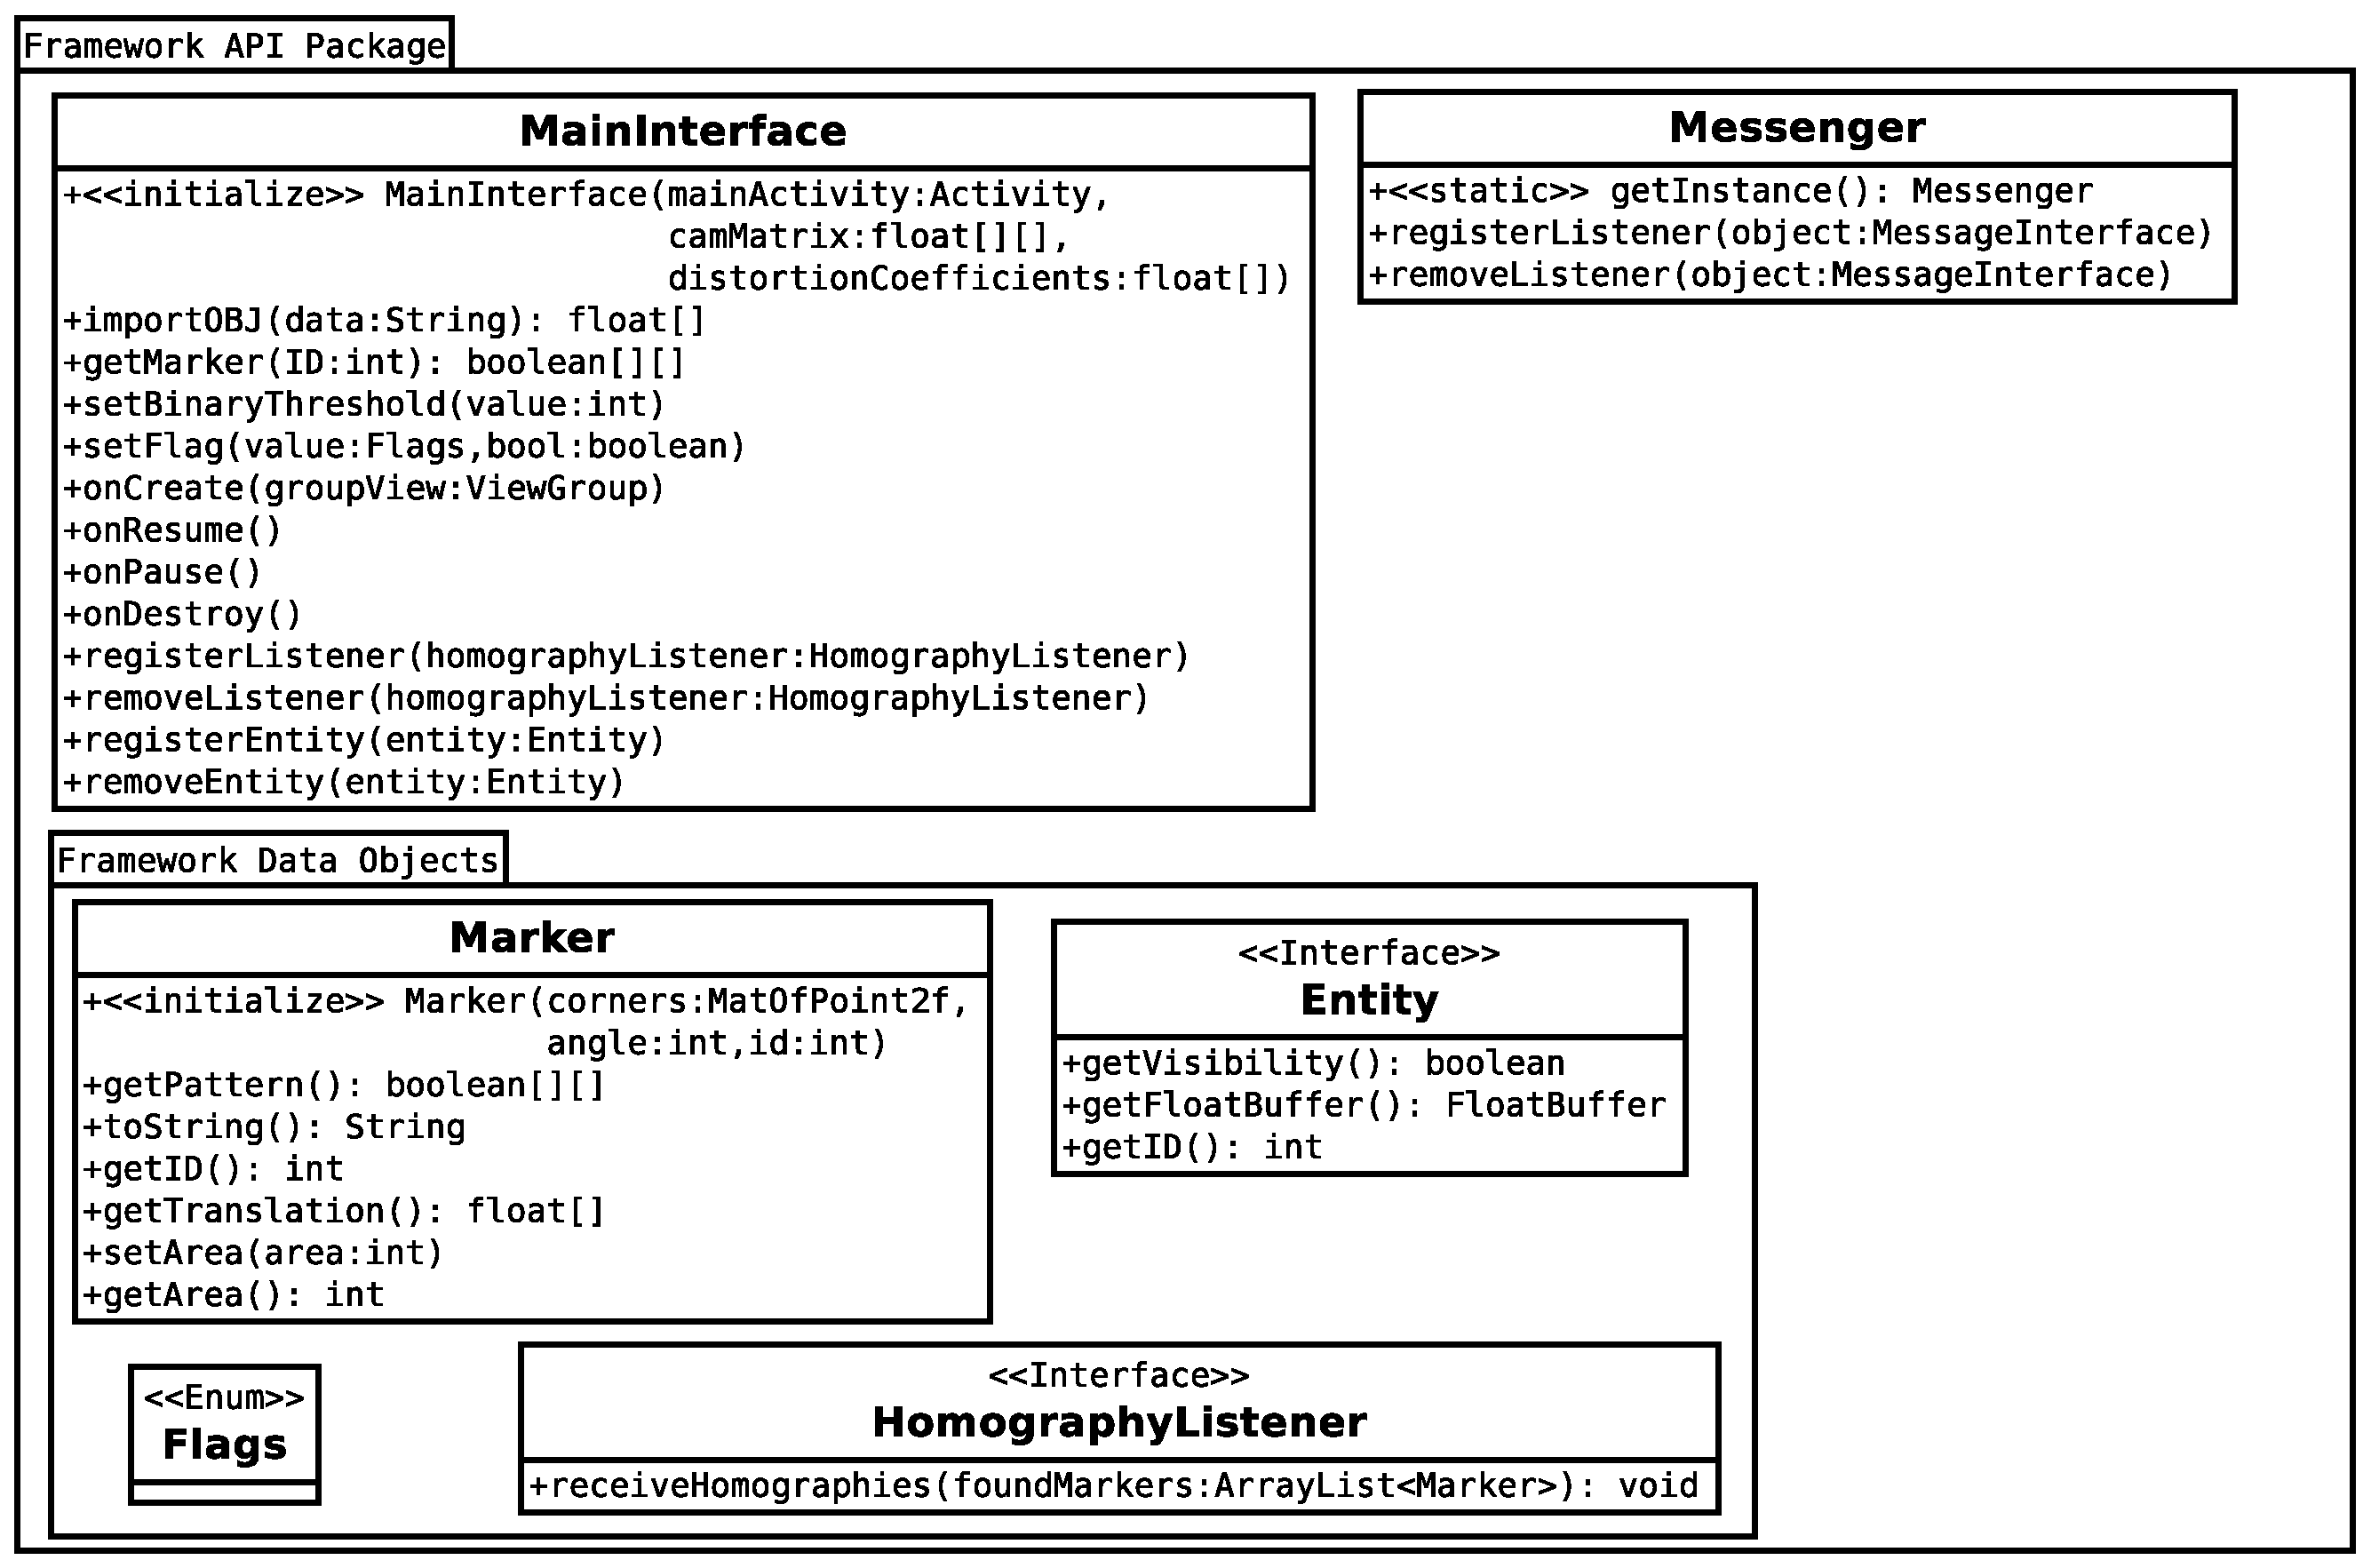
\includegraphics[width=13cm]{img/class_diagram.eps}
	\caption[Public Class Diagram]{This is the preliminary class diagram of the proposed functionality of the framework accessible from outside. It also includes data objects and interfaces required for meshing the application with Imagine.}
	\label{fig:class_diagram}
\end{figure}

Now let us take a look at the proposed class structure of the framework, as illustrated in figure \ref{fig:class_diagram}.
For the complete class diagram, see section \ref{complete_class}.

Main access is controlled over the framework controller, labeled MainInterface, which almost exclusively contains all the public methods callable from outside of the framework that matter for normal usage.
Apart from MainInterace, the log messages can be listened to via the Messenger, ConvertHelper offers Mat and float conversions, and MarkerPatternHelper offers methods for generating and detecting markers.\footnote{TAMINO TODO: See issue tracker on Github, should be consolidated into MainInterface if possible!}

Some data object classes are also accessible as public classes to ease data transfer.
Notably, this includes the Marker class for accessing the pose information and the Flags class for controlling flags for Imagine.
Interface classes are also provided for passing and receiving information.

\section{Application Programming Interface}

The following represents the methods that make up the more important aspects of the framework.
With the listed methods, all functionality that the framework offers can be accessed.

{\footnotesize
\begin{tabulary}{\textwidth}{J || J}
<<Initialization>> & Constructs all the internal classes and prepares the major functionality. Also used to set the most important values such as camera distortion and camera perspective, as these are crucial for a correct processing. Furthermore also used to set the output layout where the results are drawn to.\\
\hline
onCreate & Must be called in the activities onCreate; handles all the necessary calls within the framework.\\
\hline
onResume & Must be called in the activities onResume.\\
\hline
onPause & Must be called in the activities onPause.\\
\hline
onDestroy & Must be called in the activities onDestroy.\\
\hline
registerListener & Add a homography listener. Listeners will be called if the correct flag has been set. Listeners will receive a list of detected markers containing all information.\\
\hline
removeListener & Removes a homography listener. \\
\hline
registerEntity & Adds an entity containing the ID, visibility status, and vertice buffer. This means that upon detection of the corresponding marker, the object will be rendered on top of it, according to the status of the visibility.\\
\hline
removeEntity & Removes an entity from the list.\\
\hline
setDebugFlag & Sets the given debug flag. For possible flags please see the Javadoc.\\
\hline
removeDebugFlag & Unsets the given debug flag.\\
\end{tabulary}
}

Important to note is that the onCreate, onPause, onResume, and onDestroy methods are inherent to the way programs work on Android, and thus must be called for the framework to function correctly.

Upon initialization of the framework, entities can be added to be tracked and rendered with the registerEntity method.
To do that, the user has to implement the entity interface, providing functionality for reading the identification that the object is to be bound to, whether it is to be rendered (the visibility option), and finally a FloatBuffer containing the vertice location and color information.
The use of the FloatBuffer might not seem intuitive at first glance, however it allows the framework to handle the rendering all on its own, greatly simplifying the usage of the framework.

\section{Usage}

The finished framework can track multiple markers in a single instance.
In fact, it tracks all markers it finds from the beginning, only filtering out the ones that the user is interested in before rendering.
This allows comparatively easy use of multiple, separately tracked entities.
However, this also has a significant drawback: as the framework is computationally expensive, multiple markers can quickly degrade its performance, even if the user is only interested in a single marker – see also section \ref{performance}.

For the tracking to work, the marker must be visible to the camera.
The marker can be shown on a separate screen, printed on paper, or drawn.
The framework will then detect the presence of the marker, continue with its identification and perspective information, and finally store it as a successfully detected marker for the render interface to render.
Utilizing the thus calculated perspective information, paired with the correct object, the renderer then proceeds to render objects onto their respective markers.

\section{Implementation}

The following section describes in more detail the implementation of the framework.

\subsection{Tools and Environment}

We developed Imagine on a Linux Mint Debian Edition powered computer with the IntelliJ IDEA IDE\cite{idea}.
The development device was connected via USB debugging for rapid iterative coding.
Javadoc was written directly into the code and then generated to readable format via internal IntelliJ IDEA tools.

For further documentation, we utilized Dia\cite{dia} for generating diagrams, Umbrello\cite{umbrello} for the class diagrams, Texmaker\cite{texmaker} for \LaTeX  creation, and Git\cite{git} for revision control.

Imagine was developed with the target of running smoothly on a Nvidia Tegra 3 processor.
The development device is the Transformer Prime, a 10'' tablet from ASUS\cite{devicedev}.
This means that the framework should run smoothly on a 1.6Ghz Quadcore ARM processor rendering to a 1280 by 800 pixel screen.

\subsection{First Steps and Trials}

First we implemented a test project to experiment with OpenCV for Android to collect data on possible solutions and problems.
This test project was later worked into the finished framework once a suitable algorithm had been found.

At first, a feature-based detection approach for markers was tried.
That meant that feature detection was used on the marker, resulting in a cloud of key feature points.
These can then theoretically be located in an image from which we have likewise extracted feature points.
However, this method proved to be too computationally expensive considering that we would then still need to identify the marker and calculate the geometric information.
Initial tests only for detecting feature points in a live camera view yielded framerates below 2 frames per second.
This was deemed insufficient for a realtime use of the finished product.

Initialized by that, further detailed research turned up a better solution based on the method used by the comparable Aruco\cite{aruco} framework.
By comparing the performance of the marker-based approach of Aruco, the feature-based approach was discarded in favor of a marker-based approach, as it promised to offer a significant performance increase.

\subsection{Implemented Algorithm}
\label{detection_workflow}

This section describes in detail how we detect, identify, and calculate the perspective transformation of the markers in Imagine.
These steps are done for each frame, leveraging the image processing capabilities of OpenCV.
It results in a list of detected markers with their transformation matrices.

The first step is to reduce the color image into a binary image.
To do this, we take the gray-scaled image that we receive from OpenCV and threshold it against a constant value.
As we are interested in highly contrasted regions as our markers are monochrome, this threshold was chosen relatively low.
Alternative methods are available, but either have other drawbacks or take a longer amount of time\footnote{TAMINO TODO: Redo when done, other methods should work now too!}.

This binary image is suitable for fast detection of all contours within the image.
The detected contours are then filtered for size, as any contour that represents a marker below a certain size will be too small to safely and correctly identify.
The filtering also improves performance as it removes much contour noise, therefore decreasing our workload for further steps.
Next we calculate polynomial approximations for all remaining contours.
We can then filter the polynomial objects based on criteria for our markers.
Of these criteria there are two: only objects with four corners and those which form a convex hull are kept.

Now that we have a selection of detected perspective rectangles that might be markers, we sample all candidates for a black border.
To do this, we first have to de-warp the part of the image that is confined by the rectangles.
This is done to decrease sampling difficulty and decreases speed only by an insignificant amount.
The now square texture is then used in the following steps, of which the first is to check that the candidates have a valid black border.
Next we check for the orientation bits: if we find these, we can be comparatively sure that we have a valid marker and can continue to its identification.
If the detection of orientation fails (meaning that we do not find a pattern of three white and one black inner corner block), we consider the candidate to be invalid.
Now all that remains is the marker identification, which is done by sampling the remaining inside bits and decoding them.
This process is further detailed in section \ref{section_markers}.

One of the major advantages of the polynomial representation of the markers is that it is very easy to calculate the 3D position of the markers from them.
This is done by solving a linear equation that tries to find the translation values required to move the marker from the camera plane correctly to its 3D location according to its perspective distorted location.
That step is the one that requires the camera matrix and camera distortion values, which have to be determined beforehand for each device.
The resulting translation is saved along with marker identification and angle.
It will later be used to correctly place an object on top of the marker to be rendered in OpenGL.
All thus detected marker candidates are then passed to the main controller, which manages them for the renderer.

For further commentary on the implementation, see section \ref{implementation}.
Concerning final performance of the framework, see section \ref{performance}.

\section{Complete Class Diagram}
\label{complete_class}

Figure \ref{fig:complete_class_diagram} shows the complete class diagram of the finished framework.

MainInterface encapsulates all the primary functionality within the framework that is required to work with if from an application.
Apart from managing all the other classes on startup and closure, it also handles the information exchange between them and the application itself.
It also enables the management of the entities and their assigned trackables\footnote{TAMINO TODO: Add to glossary!}.
MainInterface also handles any inter-system compatibility that the passage of information between the renderer and interface require, such as the filtering of detected markers for trackables that are to be rendered.

The Messenger class allows easy and quick access to any debugging, logging, or error messages to outside classes via a listener principle.
This allows outside threads to be directly notified when a message is written and allows the end user to expand on any messages from the framework.

The OpenGLRenderer implements the functions that take the list of detected trackables and renders their objects onto the position given by the pose estimation.
This class also implements all functionality for the rendering types and 3D drawing functions that are required.

The OpenCVWorker is a single thread that continually takes an input image and tries to detect all markers in it.
The functionality itself however rests in the Detector class; this class only handles the logical functions surrounding the multithreading and work delegation.

The Detector class is where the main detection code lies.
The algorithm was thus extracted from other classes to allow a clean differentiation in functionality.
Here, the main OpenCV work is done.
Detector also implements a few internal methods for the detection work that would be ill suited to lay elsewhere.

\begin{sidewaysfigure}
	\centering
	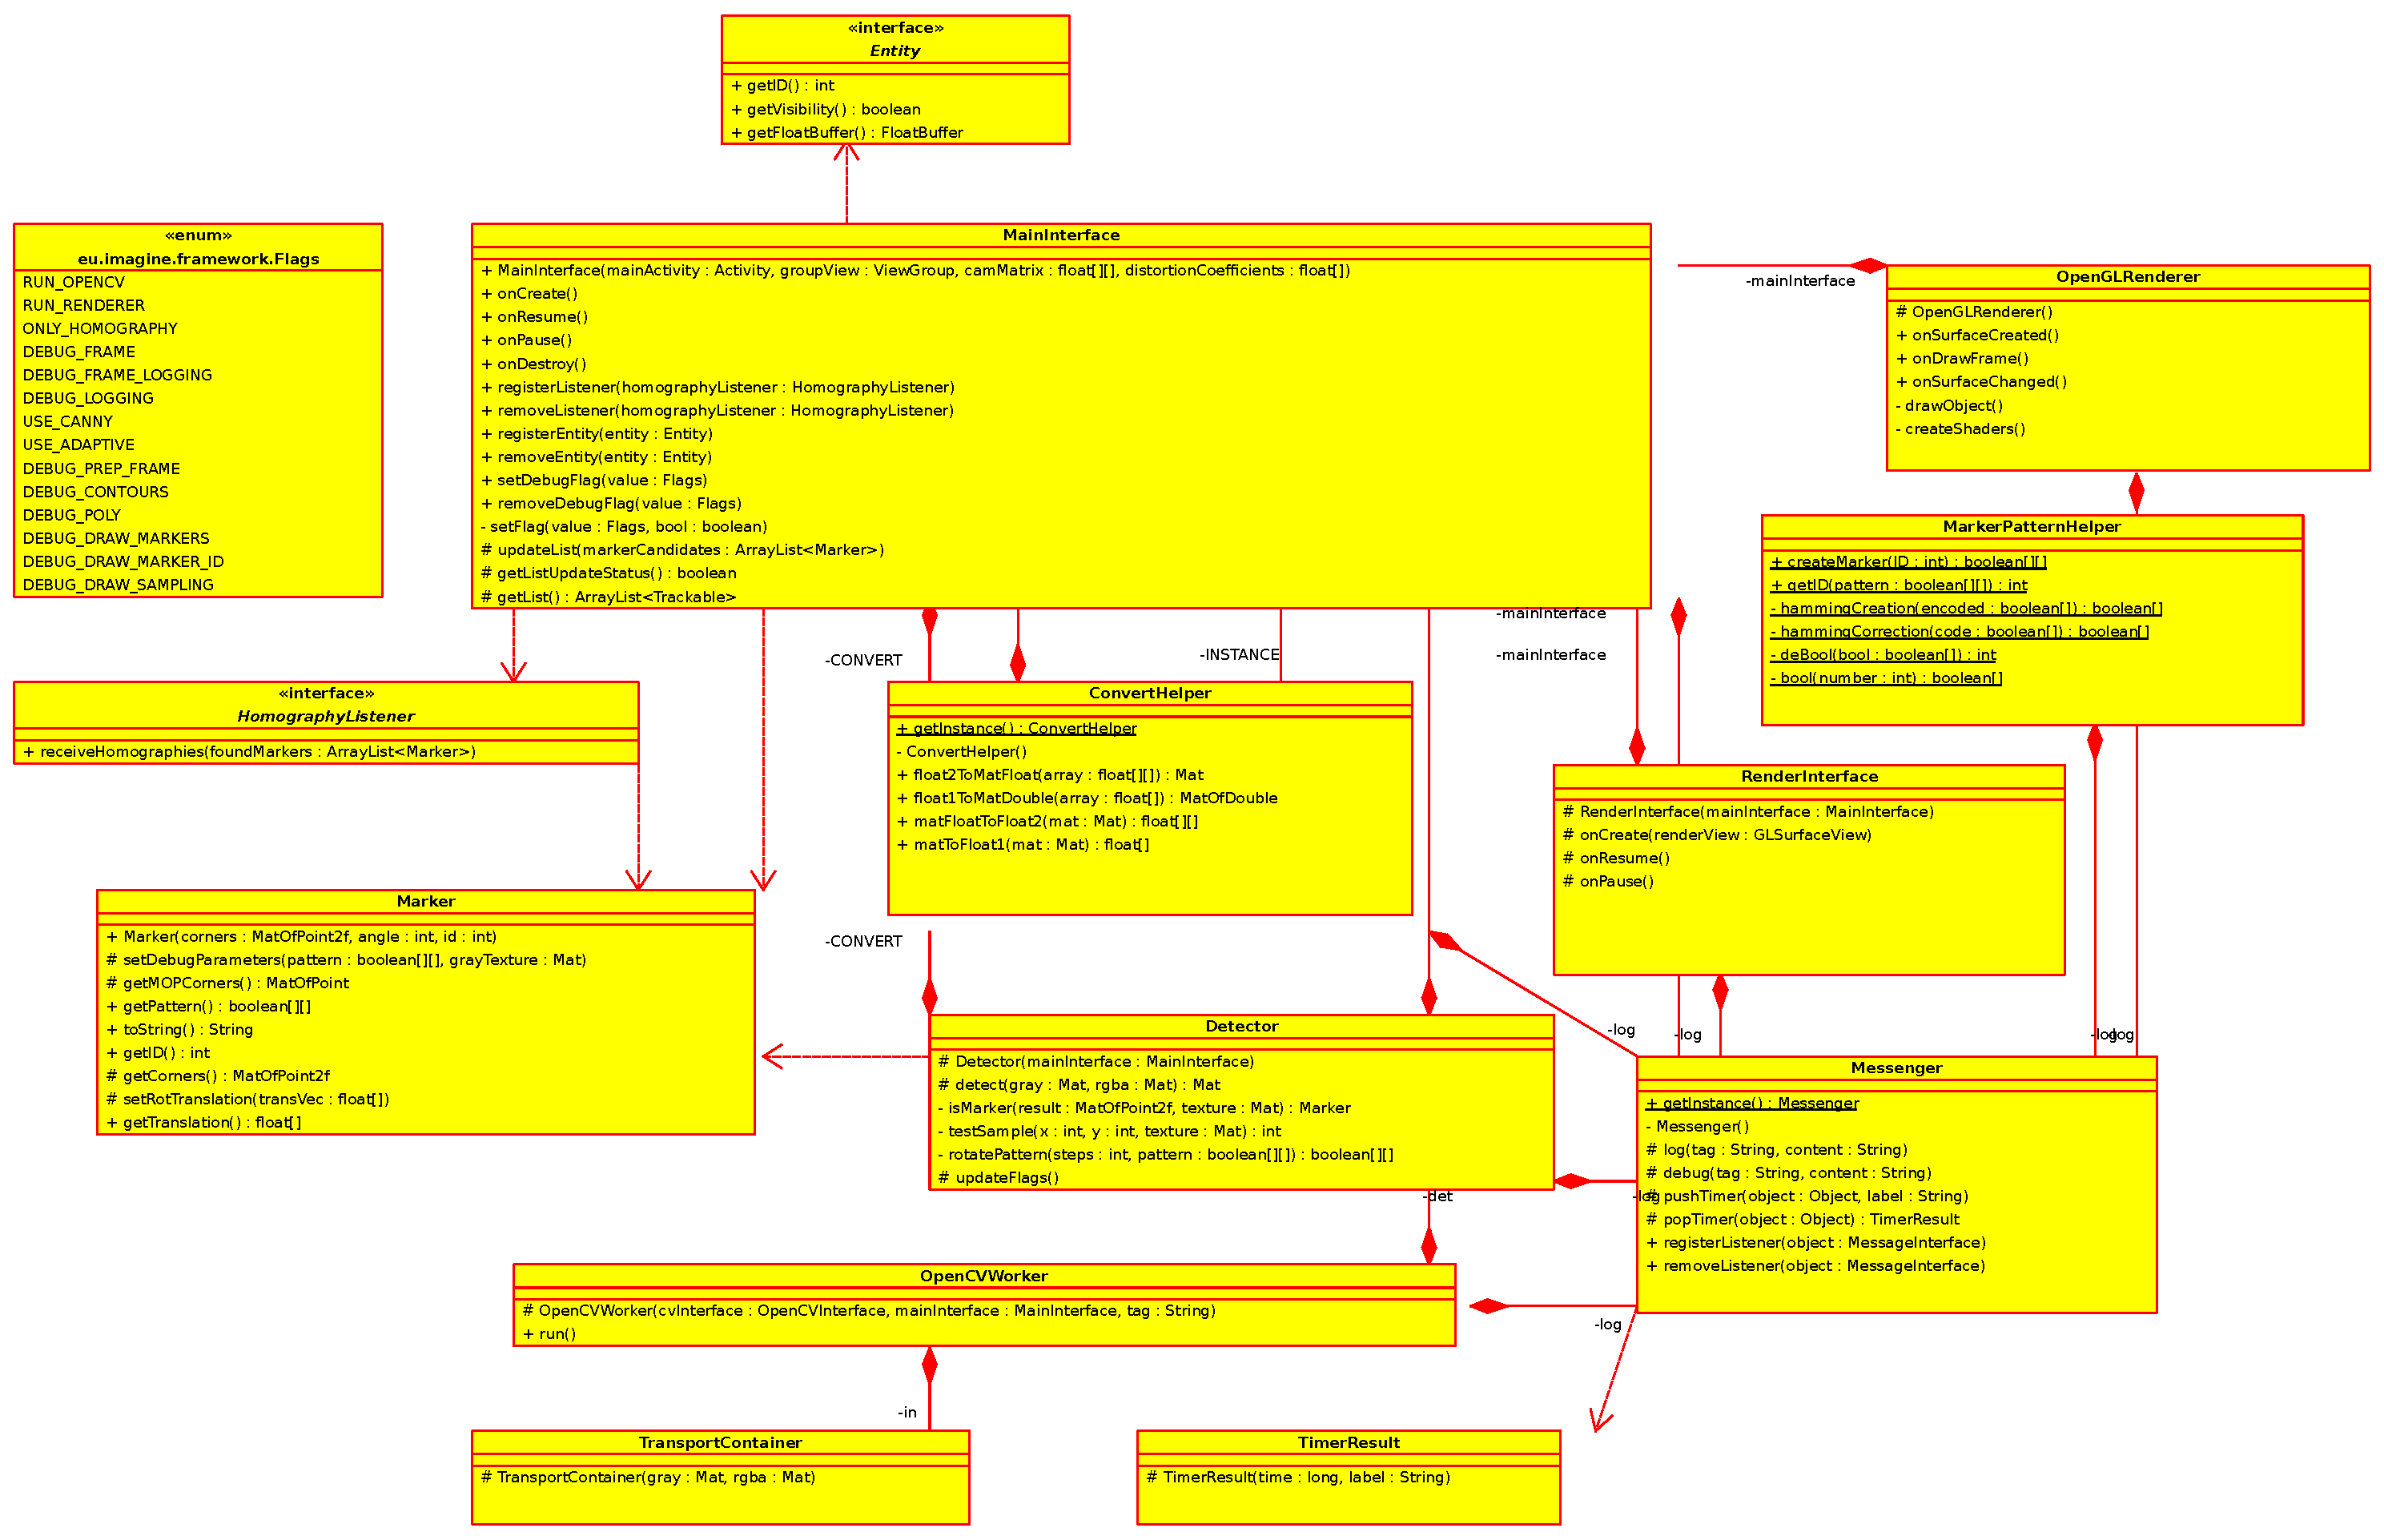
\includegraphics[width=21cm]{img/complete_class_diagram.eps}
	\caption[Complete Class Diagram]{This is the complete class diagram of the Imagine framework. It lists all methods of all the public, protected, and private classes. Attributes were left out for formatting reasons; especially the Detector class has a large amount of attributes that would not fit into this diagram.}
	\label{fig:complete_class_diagram}
\end{sidewaysfigure}

The above proposed system should enable an easily extensible build for the framework while retaining a simplistic use case.
It should, in theory, be relatively easy to exchange either the worker threads or the render class to enable the framework to run beyond Android.
That would enable the framework to run on normal personal computers using the full-fledged version of OpenGL or possibly DirectX.

\section{How to Use}

Using the framework is very easy.
Simply create an instance of the MainInterface of the framework either in the constructor or in the onCreate method of the activity where the application is run from.
After creating the instance, the onCreate method of the framework must be called from within the activity's own onCreate method.
To create the framework, an Android GroupView is required.
Here it will place the camera view and the view responsible for rendering the detected objects. Also required are the camera values for the target device.
These can either be calculated, copied from device information, or detected with an application like the following: \url{https://github.com/Itseez/opencv/tree/master/samples/android/camera-calibration}.
Now all that remains is to also call onPause, onResume, and onDestroy in the respective functions of the activity via the framework.

The framework offers some helper functions to shift some workload away from the user.
These should allow the usage of the framework to be very quick to learn and implement, without having to understand how the framework works internally.

One such helper function is the creation of correct markers in the form of a binary array.
This can be used one-off to create a printable set of markers, or during use of the framework for internal representation of markers.
The method takes the identification number and generates the complete marker for it, including border, orientation bits, and Hamming encoding.

Another helper function loads a 3D model file and converts it to the correct representation to be used with the entity class.
This method takes a 3D model file and converts it to the FloatBuffer data structure used by the framework, if capable.
